\documentclass[a4paper,12pt,landscape]{article}
\usepackage{fullpage} % for 1.5 cm margins
\renewcommand{\familydefault}{\sfdefault} % so it doesn't look like LaTeX
\usepackage{helvet}
\usepackage[british]{isodate}
\usepackage{abstract}
\renewcommand{\abstractname}{Overview}
\newcommand{\tickbox}{\framebox(12,12){} }
\newcommand{\fillbox}{\begin{tabular}{|l|}
  \hspace{60pt} \\
  \hline
\end{tabular} }
\usepackage{enumitem, amssymb} % for checklists
\newlist{todolist}{itemize}{1}
\setlist[todolist]{label=$\tickbox$, parsep=1em}
\raggedright
\raggedbottom
\usepackage{multicol}
\usepackage{graphicx}
\usepackage{parskip}

\newcommand{\documenttitle}{Shropshire Botanical Society Online Flora}
\newcommand{\documentauthor}{Joe J Collins}
\newcommand{\nbnrecords}[1]{\href{https://records-ws.nbnatlas.org/#1}{\detokenize{https://records-ws.nbnatlas.org/#1}}}
\newcommand{\wireframe}[1]{\includegraphics[width=0.85\textwidth,height=\textheight,keepaspectratio]{#1}\clearpage}

\title{Shropshire Botanical Society Online Flora\\
Web application Specification}
\author{\documentauthor}
\date{\today}

\usepackage[pdftex,
  pdftitle={\documenttitle}, 
  pdfauthor={\documentauthor},
  pdfsubject={\documenttitle}]{hyperref}

\begin{document}
\maketitle
\begin{abstract}
  \begin{center}
    \begin{minipage}{0.5\textwidth}
      \strut\\
      The Shropshire Botanical Society is seeking
      to renew it's Online Flora web application.
      This specification out lines the hoped for functionality
      together with the technical
      and
      development constraints of the work.
    \end{minipage}
  \end{center}
\end{abstract}

\newpage% Blank page behind title page
\mbox{}
\clearpage

\begin{multicols*}{2}
  \setcounter{tocdepth}{3}
  \tableofcontents
  \columnbreak

  \section{Background}
  The Shropshire Botanical Society
  has been dedicated to promoting the enjoyment,
  understanding and conservation of the flora of Shropshire
  since the 18\textsuperscript{th} century.
  One of the principle activities of the Society is to collect and maintain records 
  of plant sightings within the historical boundaries of the county of Shropshire.
  Since 2003 the Society has made these records freely available online via a bespoke web application
  or Online Flora.
  This original Online Flora was written using
  PHP and the CodeIgniter Web Framework
  backed by a MySql database.
  The web application is still available at 
  \href{https://captain-blue.azurewebsites.net/}{captain-blue.azurewebsites.net}
  but unfortunately the data is now many years out of date.

  Maintaining and updating the database has proved to be challenging.
  Additionally the application was conceived prior to the introduction of the iPhone
  and it not suited to mobile use.
  Hence the Society seeks to renew the web application,
  to provide a more modern mobile interface
  and to use up to date data stored
  by the \href{https://nbnatlas.org/}{National Biodiversity Network Atlas}.
  Currently all the Society's records are submitted to the 
  National Biodiversity Network Atlas
  and since 2017 the Society's records have been available via a web service at
  the \href{https://api.nbnatlas.org/}{NBN Web service API}.
  Using the NBN Web service API provides reliable data source
  and
  a supported service for maintaining and updating the Society's records.

  \clearpage

  \section{Objective}
  To replicate the functionality of the original Online Flora
  in a responsive mobile design
  using data sourced from the NBN Web service API.

  The Online Flora is to be used for searching the Society's records
  but not for entering new records.
  Maintaining and updating the data is conducted via a separate manual process.
  Searches of the database are conducted for three different geographical scenarios.

  \section{Context}

  \subsection{Users and Usage}
  Users of the Online Flora are typically
  members of the Society
  and
  as such are often very experienced botanists.
  In a typical scenario a member of the Society
  (intending to visit a location)
  would search for a list of species that have previously
  been sighted at a location.
  It is the community or suite of species at a location that is of most interest.
  For an experienced botanist a species list for a location
  can provide information about
  the ecology, geology and history of a location,
  but will also indicate what other species might be present but have not yet been observed.
  Ideally the member of the Society
  would also wish to drill down to see individual records of species sightings,
  with dates, attributions and further details.
  This background will give a botanist
  some insight about how much weight or credence can be given to individual sightings.

  The Online Flora will serve three scenarios for
  searching for species lists.

  \begin{description}
      \item[Search Shropshire:]
        searching all the records of based on the name of the plant.
        Allowing the user to drill down to a single sighting record
        or
        showing a map of grid squares with records for a named plant.
      \item[Search by Site:]
        searching for a named site,
        then listing the names of plants for that named site.
        Again allowing the user to drill down to a single sighting record.
      \item[Search by Monad or Grid Square:]
        Selecting a 1 km grid square within the county of Shropshire,
        then listing the names of plants for that named site.
        Again allowing the user to drill down to a single sighting record.
  \end{description}

  These three scenarios are shown in the diagram below.
  \clearpage

  \wireframe{./wireframes/Overview.png}%

  \subsection{Categories of Plants}
  Gaining experience identifying plants is a lifetimes work
  and members of the Society will often
  focus their attention on one category of plants.
  So the Society's observation records
  are separated into \textbf{vascular plants} and \textbf{bryophytes},
  (two categories within the kingdom of all plants).
  A member of the Society will often wish to limit their searches to the
  category of plants they are most interested in.

  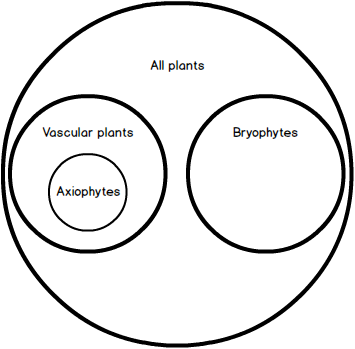
\includegraphics[width=0.4\textwidth,height=\textheight,keepaspectratio]{./wireframes/Categories.png}

  For the vascular plants
  the concept of indicator species is highlighted
  by a sub group of vascular plants
  (referred to as \textbf{axiophytes})
  These are plants that are archetypical or axiomatic for a particular ecological environment.
  So a member of the Society interested in vascular plants
  will often wish to see only the axiophytes
  to gain a better understanding of the ecological environment
  at a particular site.

  \subsection{Data Storage}
  The \href{https://nbnatlas.org/}{National Biodiversity Network Atlas}
  provides a service to maintain and distribute biological records
  for the United kingdom.


  \url{https://records.nbnatlas.org/occurrences/search?q=data_resource_uid%3Adr782}
  All the records may be searched on the NBN website. 

  a regular(ish) process in place for passing updates to the NBN.  
  
   every 6 months or so. 
   
  updating and maintaining
  The online flora/data portal will use the NBN (National Biodiversity Network) 
  as a data source and will present a filtered representation of just the SEDN 
  (Shropshire Ecological Data Network) dataset on the NBN (limited to vascular plants and bryophytes). 
  records for the entire country

  Based on Solr but with a specialised API

  The Society's records exist within
  the \href{https://registry.nbnatlas.org/public/show/dp120}{Shropshire Ecological Data Network records}.
  This dataset includes records from other recording groups in Shropshire.

  \begin{description}
    \item Cache NBN data for a month, if valid json.
      Data turn over is slow the the NBN API can be laggy. 
    \item[] 
  \end{description} 

\end{multicols*}

%%%%%%%%%%%%%%%%%%%%%%%%%%%%%%%%%%%%%%%%%%%%%%%%%%%%%%%%%%%%%%%%%%%%%%%%%%
\begin{multicols*}{2}[%
  \section{Search the County}%
  \subsection{Species List for County}%
]
\thispagestyle{empty}
\wireframe{./wireframes/Species__ListForCounty.png}%

The `landing' page for the application is the search of the entire dataset for the county.
Initially the search output should be empty.

\begin{todolist}
  \item On landing the selected list is empty.
  \item By default the \textbf{Scientific} name selected first.  
  favour identifying
  plant species via the scientific name.
  \item If \textbf{Common} set a cookie to retain the user's choice of naming type.
  \item Also set a cookie for the user's choice of plant group
\end{todolist}

\begin{todolist}

  \item The characters entered in the search box are used to search for names beginning with those letters,
    not within the names.
  \item Clicking on \textbf{list} or pressing return on the desktop list will fill the list.
  \item If \textbf{Common} is selected, only the species with common names will be searched and shown.
  \item If \textbf{Axiophytes} a limited static list of scientific names will be searched and shown.
  \item Changing the radio button will reset the search and blank the list.
\end{todolist}

e.g. \footnote{\nbnrecords{explore/group/Plants?fq=data_resource_uid:dr782+AND+taxon_name:B*}}

\subsection{Records for a Single Species in the County}

\wireframe{./wireframes/Records__SingleSpeciesForCounty.png}%

Clicking on a species name will show details for the 

\begin{todolist}
  \item Collapse the map? Retain state in cookie
  \item Page the records?
  \item Site link goes to what?
\end{todolist}

\clearpage
\subsection{A Single Record}

\wireframe{./wireframes/Records__SingleRecord.png}%

\begin{itemize}
  \item .
\end{itemize}

\end{multicols*}

%%%%%%%%%%%%%%%%%%%%%%%%%%%%%%%%%%%%%%%%%%%%%%%%%%%%%%%%%%%%%%%%%%%%%%%%%%
\begin{multicols*}{2}[%
  \section{Search in a Site}%
  \subsection{Site List for the County}%
]
\thispagestyle{empty}
\wireframe{./wireframes/Sites__ListForCounty.png}%

\begin{itemize}
  \item List is empty, actually is this necessary?
\end{itemize}

e.g. \url{https://records-ws.nbnatlas.org/occurrences/search?fq=location_id:[Church%20TO%20*]&fq=data_resource_uid:dr782&facets=location_id&facet=on&pageSize=0}
\clearpage

\subsection{Species List for a Site}

\wireframe{./wireframes/Species__ListForSite.png}%

\begin{itemize}
  \item .
\end{itemize}
\clearpage

\subsection{Records for a Single Species at a Site}

\wireframe{./wireframes/Records__SingleSpeciesForSite.png}%

\begin{itemize}
  \item .
\end{itemize}
\clearpage

\end{multicols*}

%%%%%%%%%%%%%%%%%%%%%%%%%%%%%%%%%%%%%%%%%%%%%%%%%%%%%%%%%%%%%%%%%%%%%%%%%%
\begin{multicols*}{2}[%
  \section{Search in a Square}%
  \subsection{Select a Square}%
]
\thispagestyle{empty}
\wireframe{./wireframes/Squares__Index.png}%

\begin{itemize}
  \item Zoom in and select.
  \item Graticule
\end{itemize}
\clearpage

\subsection{Species List for a Square}

\wireframe{./wireframes/Species__ListForSquare.png}%

\begin{itemize}
  \item .
\end{itemize}
\clearpage

\subsection{Records for a Single Species at a Site}

\wireframe{./wireframes/Records__SingleSpeciesForSquare.png}%

\begin{itemize}
  \item .
\end{itemize}
\clearpage

\end{multicols*}

\begin{multicols*}{2}[%
  \section{Technical Constraints}%
]

% Simple and convenient caching.
% Possible to source PHP developers from within the ranks of members.
% Possibility of free hosting on the Google App Engine.
% Simplest possible with the lowest barrier to entry.
% Almost any programmer should be able to work on it.

The Botanical Society has limited means
and wishes to ensure that the results of any programming effort
can be maintained and supported
into the future,
either via an open source project or via the efforts of members of the Society.
To facilitate these possibilities
the technical environment for the projects is intended 
to provide a low barrier to contributions.

\begin{description}
    \item[PHP 7.3] for deployment to Google App Engine for free hosting.
    \item[CodeIgniter 4.0.4] has been used successfully in the past and provides convenient caching should it be required.
    \item[Twitter Bootstrap 4.5.2] for responsive layout.
    \item[Leaflet 1.6.0] should be used to provide mapping services.
     https://github.com/DuncanRowland/NBNMapOverlayExamples
    \item[Commits to Github] since the Society will retain the intellectual property rights
      over any code produced.
      So all branching should be on the repository at
      at \href{https://github.com/joejcollins/captain-magenta.git}{Github}
      The Society will
    \item[Style Sheet] taken from \href{https://www.shropshirebotany.org.uk/}{www.shropshirebotany.org.uk}.
      The Online Flora is to be consistent with this website,
      so should reuse the same classes and styles.
    \item[No NBN API Calls from the Client] because we might want to use caching.
    \item[No database] should be used other than the NBN Web service API.
      Any static data 
      (such as the list of axiophytes)
      should be hard coded into the application.
\end{description}

\end{multicols*}



\end{document}


